\documentclass[final]{beamer}
\usepackage[utf8]{inputenc}
\usepackage[T1]{fontenc}

\usepackage{helvet}

\usepackage{listings}
\usepackage{graphicx}
\usepackage[export]{adjustbox}
\usepackage{tikz}
\usetikzlibrary{calc}

\usepackage{subcaption}
\captionsetup{compatibility=false}

\renewcommand*{\tiny}{\fontsize{10pt}{12pt}\selectfont}
\newcommand*{\authorsize}{\fontsize{14pt}{16pt}\selectfont}
\renewcommand*{\scriptsize}{\fontsize{18pt}{20pt}\selectfont}
\renewcommand*{\footnotesize}{\fontsize{20pt}{22pt}\selectfont}
\renewcommand*{\small}{\fontsize{24pt}{26pt}\selectfont}
\renewcommand*{\normalsize}{\fontsize{28pt}{30pt}\selectfont}
\renewcommand*{\large}{\fontsize{30pt}{32pt}\selectfont}
\renewcommand*{\Large}{\fontsize{30pt}{32pt}\selectfont}
\renewcommand*{\LARGE}{\fontsize{32pt}{34pt}\selectfont}
\renewcommand*{\huge}{\fontsize{34pt}{36pt}\selectfont}
\renewcommand*{\Huge}{\fontsize{36pt}{38pt}\selectfont}

\definecolor{dkgreen}{rgb}{0,0.6,0}
\definecolor{gray}{rgb}{0.5,0.5,0.5}
\definecolor{mauve}{rgb}{0.58,0,0.82}
\definecolor{ornlgreen}{rgb}{0.11765, 0.46275, 0.25098}
\definecolor{ornllightgreen}{HTML}{84B641}

\lstset{
  language=C,                     % the language of the code
  %basicstyle=\footnotesize,
  basicstyle=\ttfamily\scriptsize,      % the size of the fonts that are used for the code
  numbers=left,                   % where to put the line-numbers
  numberstyle=\tiny\color{gray},  % the style that is used for the line-numbers
  stepnumber=1,                   % the step between two line-numbers. If it's 1, each line
                                    % will be numbered
%  backgroundcolor=\color{white},  % choose the background color. You must add \usepackage{color}
  showspaces=false,               % show spaces adding particular underscores
  showstringspaces=false,         % underline spaces within strings
  showtabs=false,                 % show tabs within strings adding particular underscores
  rulecolor=\color{black},        % if not set, the frame-color may be changed on line-breaks within not-black text (e.g. commens (green here))
  tabsize=2,                      % sets default tabsize to 2 spaces
  captionpos=b,                   % sets the caption-position to bottom
  breaklines=true,                % sets automatic line breaking
  breakatwhitespace=true,        % sets if automatic breaks should only happen at whitespace
  %title=\lstname,                 % show the filename of files included with \lstinputlisting;
  %caption=\lstname,                                 % also try caption instead of title
  keywordstyle=\color{blue},          % keyword style
  commentstyle=\color{dkgreen},       % comment style
  stringstyle=\color{mauve},         % string literal style
  escapeinside={\%*}{*)},            % if you want to add LaTeX within your code
  xleftmargin=15pt,
  morekeywords={*,...}              % if you want to add more keywords to the set
}
\lstset{numbers=left,numberblanklines=false,escapeinside=||}

\geometry{papersize={33.857847cm, 19.05cm}}

\setbeamercolor{frametitle}{fg=ornlgreen}

\addtobeamertemplate{frametitle}{%
	\vspace{0.06\paperheight}
}

\makeatletter

\newcommand\emuwidth{\convertto{cm}{\paperwidth} * 360000}
\newcommand\emuheight{\convertto{cm}{\paperheight} * 360000}
\newcommand\curvestretch{0.971599}
\newcommand\bigcurvestretch{0.971530}

\newcommand\DrawControl[3]{node[#2,circle,fill=#2,inner sep=2pt,label={above:$#1$},label={[black]below:{\footnotesize#3}}] at #1 {}}

\usebackgroundtemplate{%
%    \includegraphics[width=0.5\paperwidth,height=\paperheight]{images/isaac_newton-282x300.jpg}%
	\ifnum\c@framenumber=1%
%	\begin{tikzpicture}[remember picture, overlay, fill opacity=0.35, draw opacity=1]%
%	\draw[ornllightgreen, fill=ornllightgreen] ($ (current page.north west) + (0.752424\paperwidth, -0.498449\paperheight) $) circle (0.088265\paperwidth);
%	\draw[ornllightgreen, fill=ornllightgreen] ($ (current page.north west) + (0.867464\paperwidth, -0.543115\paperheight) $) circle (0.076628\paperwidth);
%	\draw[ornllightgreen, fill=ornllightgreen] ($ (current page.north west) + (0.789000\paperwidth, -0.705333\paperheight) $) circle (0.068250\paperwidth);
%	\end{tikzpicture}
	\begin{tikzpicture}[remember picture, overlay, complexnode/.pic={\draw[color=ornlgreen, fill=ornlgreen] (0, 0) .. controls (0, 0) and (304 * \bigcurvestretch / 2166, -816 / 2166) .. (150 * \bigcurvestretch / 2166, -1) -- (1, -1) -- (1, 0) -- (0, 0);}, othernode/.pic={\draw[ultra thick, color=ornllightgreen, fill=ornllightgreen] (0, 0) .. controls (0, 0) and (346 * \curvestretch / 2166, -767 / 2166) .. (221 * \curvestretch / 2166, -1) -- (240 * \curvestretch / 2166, -1) .. controls (240 * \curvestretch / 2166, -1) and (402 * \curvestretch / 2166, -989 / 2166) .. (90 * \curvestretch / 2166, 0) -- (0, 0);}]%
%	\draw[help lines] (0, 0) grid (8, 5);
	\draw (0.643489\paperwidth, 0) pic[scale=7.5 * 2.54] {complexnode};
	\draw (0.619382\paperwidth, 0) pic[scale=7.5 * 2.54] {othernode};
%	\draw[fill=ornlgreen] (0, 0) -- (10, 0) -- (10, -10) -- (0, -10) -- (0, 0);
%	\draw[ultra thick, blue] (1, 0) .. controls (4, 2) .. (7, 0) \DrawControl{(4, 2)}{blue}{};
%	\draw[ultra thick, red] (1, 0) .. controls (4, 6) .. (7, 0) \DrawControl{(4, 6)}{blue}{};
	\end{tikzpicture}
	\begin{tikzpicture}[shift={(current page.north west)}, remember picture, overlay]%
%	\node[anchor=north west, inner sep=0] at (0.575892\paperwidth, -0.184615\paperheight) {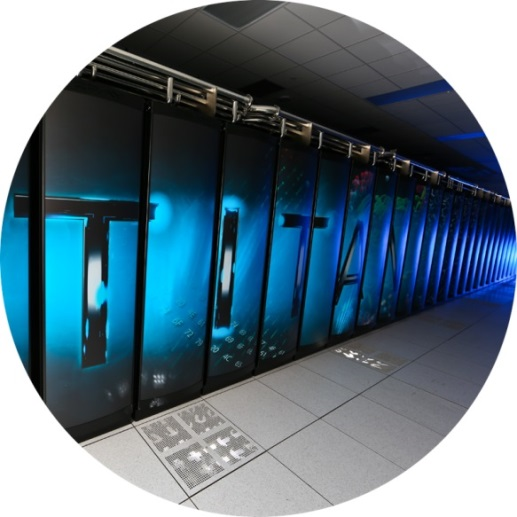
\includegraphics[width=0.176531\paperwidth, height=0.176531\paperwidth]{images/titan-bubble.jpeg}};%
	\node[anchor=north west, inner sep=0, minimum size=0.176531\paperwidth, circle, path picture={\node at (path picture bounding box.north west) {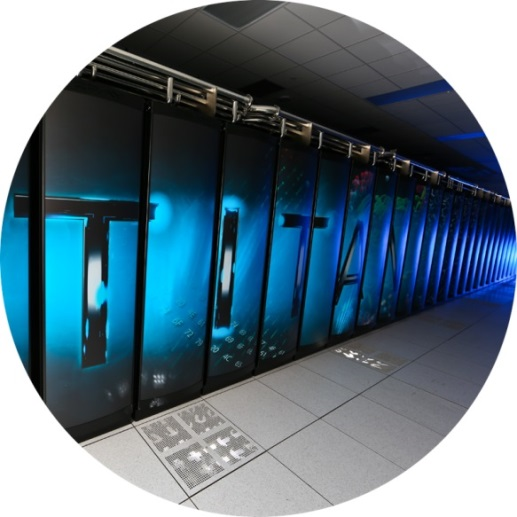
\includegraphics[width=0.176531\paperwidth, height=0.176531\paperwidth]{images/titan-bubble.jpeg}};}, draw=ornllightgreen, line width=6pt, draw opacity=0.65] at (0.575892\paperwidth, -0.184615\paperheight) {};%
%	\draw[ultra thick, red] (0, 0) -- (0.57892\paperwidth, -0.184615\paperheight);
	\node[anchor=north west, inner sep=0, minimum size=0.153256\paperwidth, circle, path picture={\node at (path picture bounding box.north west) {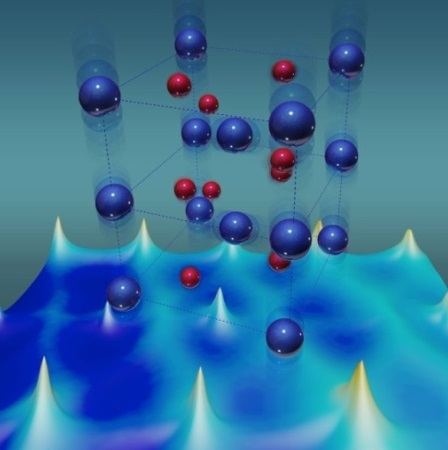
\includegraphics[width=0.153256\paperwidth, height=0.153256\paperwidth]{images/particles.jpeg}};}, draw=ornllightgreen, line width=6pt, draw opacity=0.65] at (0.714207\paperwidth, -0.270660\paperheight) {};%
	\node[anchor=north west, inner sep=0, minimum size=0.136500\paperwidth, circle, path picture={\node at (path picture bounding box.north west) {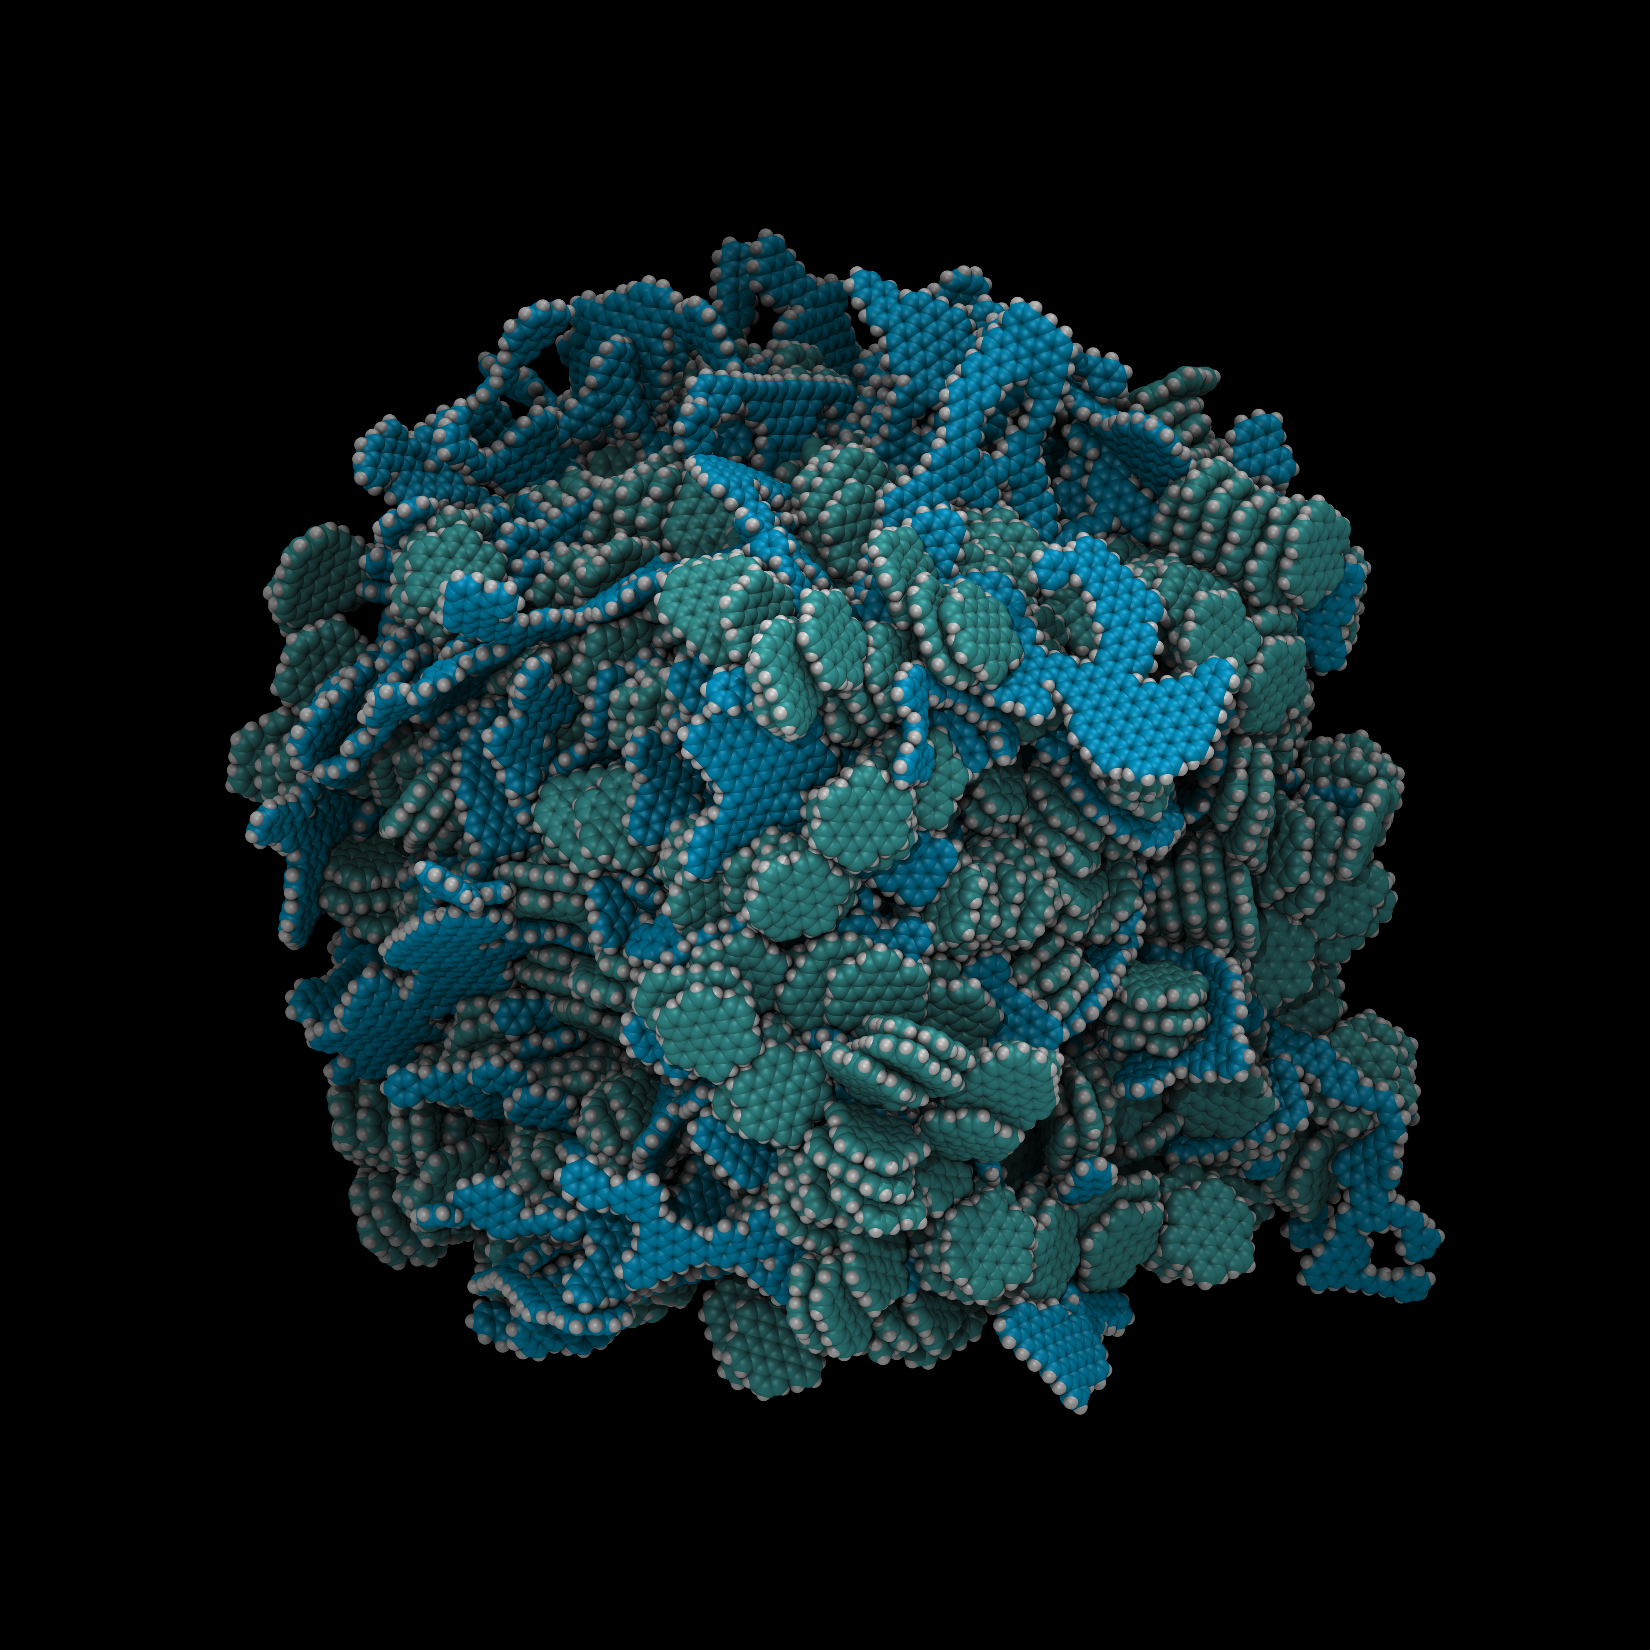
\includegraphics[width=0.136500\paperwidth, height=0.136500\paperwidth]{images/scimari.png}};}, draw=ornllightgreen, line width=6pt, draw opacity=0.65] at (0.652500\paperwidth, -0.462666\paperheight) {};%
%	\fill[ornlgreen] (0.7\paperwidth, 0) rectangle (\paperwidth, -\paperheight);
	\node[anchor=north east, inner sep=0] at (current page.north east) {
\includegraphics[width=0.725\paperwidth, height=0.967\paperheight]{images/nucleus.png}};%
    \node[xscale=-1, anchor=north east, inner sep=0] at (current page.north west) {\adjincludegraphics[trim={0.53723\width, 0, 0.05491\width, 0.46829\height}, clip, origin=center, angle=90, width=0.347\paperwidth, height=0.631\paperheight]{images/wavegrid.png}};%
%    \node[anchor=north west, inner sep=0] at ($ (current page.north west) + (0.589\paperwidth, -0.096\paperheight) $) {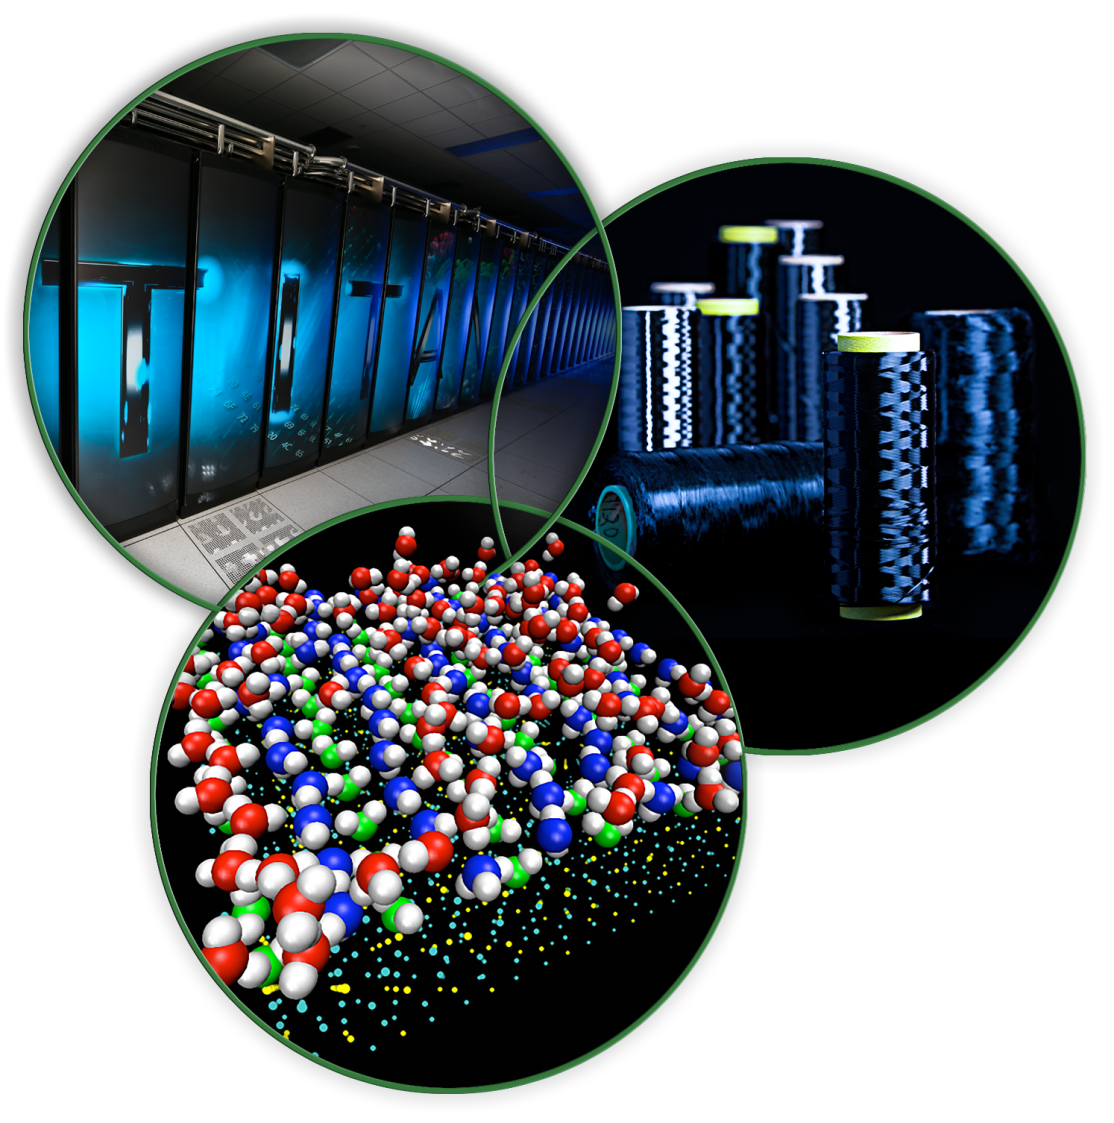
\includegraphics[width=0.38\paperwidth, height=0.68\paperheight]{images/scibubbles.png}};%
    \end{tikzpicture}%
    \else%
    \begin{tikzpicture}[remember picture, overlay]%
    \node[anchor=south east, inner sep=0] at (current page.south east) {\adjincludegraphics[trim={0.47067\width, 0, 0, 0.13722\height}, clip, width=0.416\paperwidth, height=0.905\paperheight]{images/wavegrid.png}};%
%    \node[anchor=north west, inner sep=0] at (current page.north west) {\adjincludegraphics[trim={0.53723\width, 0, 0.05491\width, 0.46829\height}, clip, origin=center, angle=90, width=0.347\paperwidth, height=0.631\paperheight]{images/wavegrid.png}};%
    \end{tikzpicture}%
    \fi%
}

\setbeamertemplate{footline}{%
	\color{gray}%
	\begin{flushleft}%
	\hspace{0.02\paperwidth}%
	\the\c@framenumber%
	\hspace{0.02\paperwidth}%
	\ifnum\c@framenumber=1%
	\color{ornlgreen}%
	\parbox{0.2\textwidth}{ORNL is managed by UT-Battelle\\%
	for the US Department of Energy}%
	\else%
	Feedback-directed optimisations to control memory placement and affinity%
	\fi%
	\vspace{0.02\paperheight}%
	\end{flushleft}%
	\begin{tikzpicture}[remember picture, overlay]%
	\ifnum\c@framenumber=1%
		\node[anchor=south west, inner sep=0] at ($ (current page.south west) + (0.853\paperwidth, 0.039\paperheight) $) {
\includegraphics[width=0.109\paperwidth, height=0.047\paperheight]{images/ORNL_Two-line_white.png}};%
	\else%
		\node[anchor=south west, inner sep=0] at ($ (current page.south west) + (0.853\paperwidth, 0.039\paperheight) $) {
\includegraphics[width=0.109\paperwidth, height=0.047\paperheight]{images/ORNL_Two-line_color.png}};%
	\fi%
%	\node[anchor=south east, inner sep=0] at ($ (current page.south west) + (0.833\paperwidth, 0.039\paperheight) $) {\includegraphics[height=0.047\paperheight]{images/logo-uh-wordmark-primary-reversed.png}};%
	\end{tikzpicture}%
}

\makeatother

\setbeamertemplate{caption}[numbered]
\setbeamertemplate{itemize item}[circle]
\setbeamertemplate{itemize subitem}{-}

\beamertemplatenavigationsymbolsempty

\let\olditem\item
%\renewcommand{\item}{\addtolength{\itemsep}{0.5\baselineskip}\olditem}
\renewcommand{\item}{\vspace{\fill}\olditem}

\usepackage[nolist]{acronym}
%\ProvideAcroEnding{possessive}{'s}{'s}
%\ExplSyntaxOn
%\NewAcroCommand \acg{
%	\acro_possessive:
%	\acro_use:n{#1}
%}
%\ExplSyntaxOff
\begin{acronym}
\acro{AMO}{atomic memory operation}
\acro{AMR}{adaptive mesh refinement}
\acro{API}{Application Programming Interface}
\acrodefplural{API}[APIs]{Application Programming Interfaces}
\acro{CAF}{Coarray Fortran}
\acro{CAS}{compare and swap}
\acro{CPU}{central processing unit}
\acrodefplural{CPU}[CPUs]{central processing units}
\acrodefplural{CRDP}[CRDP]{Computational Research and Development Programs}
\acro{CSV}{comma-separated values}
\acro{DoD}{Department of Defense}
\acro{ESSC}{Extreme Scale Systems Center}
\acro{GCC}{GNU Compiler Collection}
\acro{GPU}{graphics processing unit}
\acrodefplural{GPU}[GPUs]{graphics processing units}
\acro{HBM}{high bandwidth memory}
\acro{HCA}{host channel adapter}
\acro{IR}{intermediate representation}
\acro{MPI}{Message Passing Interface}
\acro{NUMA}{non-uniform memory access}
\acro{NVM}{non-volatile memory}
\acro{OFA}{Open Fabrics Alliance}
\acro{OLCF}{Oak Ridge Leadership Computing Facility}
\acro{ORNL}{Oak Ridge National Laboratory}
\acro{PE}{processing element}
\acro{PGAS}{Partitioned Global Address Space}
\acro{RDMA}{remote direct memory access}
\acro{RMA}{remote memory access}
\acro{SHOC}{Scalable Heterogeneous Computing}
\acro{SIMD}{single instruction, multiple data}
\acro{SPMD}{single program, multiple data}
\acro{SQL}{Structured Query Language}
\acro{UCP}{UC-Protocols}
\acro{UCS}{UC-Services}
\acro{UCT}{UC-Transports}
\acro{UCX}{Unified Communication X}
\acro{XML}{Extensible Markup Language}
\acro{XSLT}{Extensible Stylesheet Language Transformations}
\end{acronym}


\title{On Synchronisation and Memory Reuse in OpenSHMEM}
\author{Aaron Welch\inst{1}, Manjunath Gorentla Venkata\inst{1}}
\institute{Extreme Scale Systems Center\\
Oak Ridge National Laboratory\\
\email{\{welchda, manjugv\}@ornl.gov}
%\inst{1} Department of Computer Science, University of Houston, Houston, TX\\[0.3ex]
%\inst{2} High Performance Computing Research Program, Oak Ridge National Laboratory, Oak Ridge, TN\\[0.3ex]
%\inst{3} Computer Science and Mathematics Division, Oak Ridge National Laboratory, Oak Ridge, TN
}
\date{\today}

%\let\tempone\itemize
%\let\temptwo\enditemize
%\renewenvironment{itemize}{\tempone\addtolength{\itemsep}{5\baselineskip}}{\temptwo}

\begin{document}

\begin{frame}{\hspace{0.02\paperwidth}Feedback-directed optimisations to control\\\hspace{0.02\paperwidth}memory placement and affinity on\\\hspace{0.02\paperwidth}shared memory programming models}
Aaron Welch, Oscar Hernandez,\\Thaleia Dimitra Doudali, Ada Gavrilovska,\\Barbara Chapman
\end{frame}

\begin{frame}{\hspace{0.02\paperwidth}Background and Motivation}
\begin{itemize}
\item Memory hierarchies are becoming increasingly complex and are constantly evolving
\item It is unclear how to address placement for memory across these hierarchies
\item As porting code can be costly, we need to explore partially or fully automated methods for identifying memory intensive regions of code and where to focus attention on porting efforts
\item This work explores such a method, by combining information from the compiler with profiling data to analyse code using an \acs{SQL} database
\end{itemize}
\end{frame}

\begin{frame}{\hspace{0.02\paperwidth}Previous Work - CoMerge}
\begin{itemize}
\item Memory sharing schema that maximises hardware utilisation and performance across collocated applications
\item Focused on prioritising allocations of critical data objects across the memory hierarchy
\item Assumes hybrid system with two memory components
\begin{itemize}
\item FastMem - good performance, limited space (DRAM)
\item SlowMem - 0.2x bandwidth and 5x latency of FastMem, higher capacity (\acs{NVM})
\end{itemize}
\end{itemize}
\end{frame}

\begin{frame}{\hspace{0.02\paperwidth}Previous Work - CoMerge}
\begin{itemize}
\item One test run for each data object being the sole resident in FastMem
\item Performance measured by reduction from ideal case (all data in FastMem)
\item Relative performance benefits for each data object used to create priority order ranking
\item Objects are allocated in order of priority until FastMem exhausted
\end{itemize}
\end{frame}

\begin{frame}{\hspace{0.02\paperwidth}Drawbacks of CoMerge}
\begin{itemize}
\item Not automated - each test run requires manual modification of code
\item Not scalable - manual process becomes intractible with substantial numbers of data objects
\item Not generic - requires developer knowledge of the code for necessary modifications
\end{itemize}
\end{frame}

\begin{frame}{\hspace{0.02\paperwidth}Proposed Solution}
\begin{itemize}
\item Design new tool for analysing application code
\item Combine information from the compiler with data obtained through dynamic profiling
\begin{itemize}
\item Dynamic sampling provides insight into actual runtime characteristics and non-functional quality attributes
\item Compiler provides massive and detailed static information on the code and functional quality attributes
\end{itemize}
\item Organise all data into an \acs{SQL} database to enable complex investigative queries
\end{itemize}
\end{frame}

\begin{frame}{\hspace{0.02\paperwidth}Proposed Solution}
\begin{itemize}
\item Benefits
\begin{itemize}
\item Same process is scalable to code of any size
\item Only requires compiling and running the code once
\item Far greater amount of information available with which to inspect and reason about the code and its performance characteristics
\end{itemize}
\item Drawbacks
\begin{itemize}
\item Less accuracy
\item Requires user participation for analysis
\end{itemize}
\end{itemize}
\end{frame}

\begin{frame}{\hspace{0.02\paperwidth}Analysis}
\begin{itemize}
\item Extract data from \acs{GCC} compiler using plugin framework
\begin{itemize}
\item Focus on high level \acs{IR} - \acs{AST}
\item Directly translate \acs{GCC} internal data structures to database
\end{itemize}
\item Obtain run-time information from ARM MAP
\begin{itemize}
\item Samples collected every time interval
\item Extract file and line numbers for each stack frame for each process/thread for each sample
\end{itemize}
\item Combine static and dynamic information based on frequencies seen for each file and line combination
\item Using sampled frequencies to direct focus, perform queries on data structure use across visited lines
\end{itemize}
\end{frame}

\begin{frame}{\hspace{0.02\paperwidth}Analysis - Extracting Static Information}
\begin{itemize}
\item Each \acs{GCC} data structure represented as a table
\item Data members similarly directly translated as columns
\item Instances of data structures become rows in the table, keyed by address in memory and a build ID unique to the invocation of \acs{GCC}
\item Pointers to other data strucutres stored by address value for referencing and linking to other tables' keys
\end{itemize}
\end{frame}

\begin{frame}{\hspace{0.02\paperwidth}Analysis - Extracting Dynamic Data}
\begin{itemize}
\item MAP used for sampling based profiling - it stops all processes and threads in the application on consistent time intervals for sampling basic information and produces an \acs{XML} file containing the sample data when run on application
\item Each sample contains a set of distinct stacks and the number of processes/threads observed with each stack in the sample
\item We process the \acs{XML} file to extract these stacks and counts using \acs{XSLT} and insert it into a table in the database containing a unique ID for the profile, the file and line numbers as arrays of increasing depth, and the process count
\end{itemize}
\end{frame}

\begin{frame}{\hspace{0.02\paperwidth}Performing the Analysis - Imitating CoMerge}
\begin{itemize}
\item To mimic the results of our past manual analysis, for each sample we look at the deepest part of the stack, within the kernels, and count the number of samples for each file and line combination
\item We join this data to the static information from the compiler to find all statements existing on those lines
\item We further determine all read/write references to symbols within those code lines
\item We count the total number of references across the samples to each unique symbol
\item Finally, we find the symbol with the largest reference count and divide all symbol counts by that value to approximate the relative "benefit"
\end{itemize}
\end{frame}

\begin{frame}{\hspace{0.02\paperwidth}Performing the Analysis - Imitating CoMerge}
\begin{itemize}
\item Tests were run on five of the benchmarks from PolyBench - adi, doitgen, fdtd-2d, jacobi-2d-imper, and trmm
\item PolyBench is a collection of benchmarks with static control flow, extracted from operations in various domains including linear algebra, image processing, and physics simulations
%TODO taking this stuff out?
%\item Possible to enhance analysis by using polyhedral analysis
\item All tests were run with a single processor and thread
\item Timing results from our manual analysis were adjusted such that they were also relative to that of the test run with the slowest performance
\end{itemize}
\end{frame}

\begin{frame}{\hspace{0.02\paperwidth}Performing the Analysis - Imitating CoMerge}
\begin{table}[hbt!]
\begin{center}
\begin{subtable}{.45\linewidth}
\begin{tabular}{|c|c|c|}
\hline
Symbol & Actual & Predicted \\
\hline\hline
X & 1 & 0.91 \\
\hline
B & 0.85 & 1 \\
\hline
A & 0.55 & 0.77 \\
\hline
\end{tabular}
\caption{adi}
\end{subtable}
\begin{subtable}{.45\linewidth}
\begin{tabular}{|c|c|c|}
\hline
Symbol & Actual & Predicted \\
\hline\hline
cFour & 1 & 1 \\
\hline
sumA & 0.78 & 0.75 \\
\hline
a & 0.19 & 0.50 \\
\hline
\end{tabular}
\caption{doitgen}
\end{subtable}
\begin{subtable}{.45\linewidth}
\begin{tabular}{|c|c|c|}
\hline
Symbol & Actual & Predicted \\
\hline\hline
hz & 1 & 1 \\
\hline
ey & 0.77 & 0.72 \\
\hline
ex & 0.60 & 0.71 \\
\hline
\end{tabular}
\caption{fdtd-2d}
\end{subtable}
\begin{subtable}{.45\linewidth}
\begin{tabular}{|c|c|c|}
\hline
Symbol & Actual & Predicted \\
\hline\hline
a & 1 & 1 \\
\hline
b & 0.95 & 0.27 \\
\hline
\end{tabular}
\caption{jacobi-2d-imper}
\end{subtable}
\begin{subtable}{.45\linewidth}
\begin{tabular}{|c|c|c|}
\hline
Symbol & Actual & Predicted \\
\hline\hline
b & 1 & 1 \\
\hline
a & 0.04 & 0.40 \\
\hline
\end{tabular}
\caption{trmm}
\end{subtable}
%\caption{Memory Hotspot Predictions}
\label{tbl:results}
\end{center}
\end{table}
\end{frame}

\begin{frame}{\hspace{0.02\paperwidth}Performing the Analysis - CP2K}
\begin{itemize}
\item CP2K is a quantum chemistry and solid state physics software package that can perform atomistic simulations of solid state, liquid, molecular, periodic, material, crystal, and biological systems
\item Written in Fortran 2003 and supports OpenMP, \acs{MPI}, and CUDA
%\item Contains roughly 600,000 statements, 2.4 million expressions, and 740,000 symbols
\item Here we investigate CP2K's \ac{DFT} method on an OpenMP + \acs{MPI} build using 1 \acs{MPI} process and 1, 2, 4, and 8 threads
\end{itemize}
\end{frame}

\begin{frame}{\hspace{0.02\paperwidth}Performing the Analysis - CP2K DFT}
\begin{itemize}
\item We start by using the same process used in our PolyBench analysis to tally all occurrences of each symbol
\item We filter based upon symbols being referenced within a few of the top functions of interest that we want to analyse
\item We further select based upon which symbols seen are within openmp parallel and parallel do sections
\end{itemize}
\end{frame}

\begin{frame}{\hspace{0.02\paperwidth}Performing the Analysis - CP2K DFT}
\begin{center}
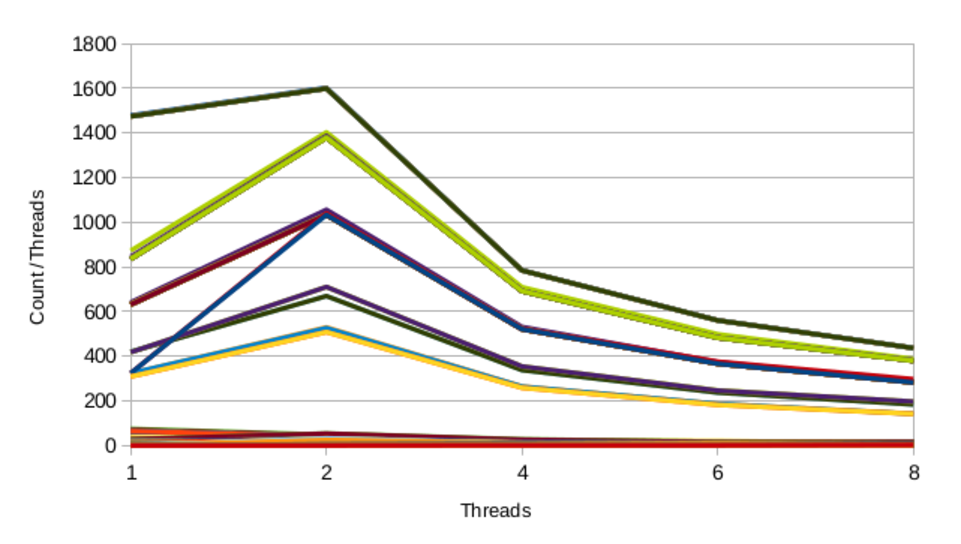
\includegraphics{images/cp2k-omp-counts.pdf}
\end{center}
\begin{itemize}
\item Each line represents a distinct symbol
\end{itemize}
\end{frame}

\begin{frame}{\hspace{0.02\paperwidth}Performing the Analysis - CP2K DFT}
\begin{itemize}
\item next chart(s) need to be described then placed here...once I can finally determine what they should be and obtain them...
\end{itemize}
\end{frame}

\begin{frame}{\hspace{0.02\paperwidth}Conclusions}
\begin{itemize}
\item Using the information combined from the compiler and profiling samples provides information about the execution of code at a previously unprecedented granularity for a relatively low overhead cost
\item Ability to query highly complex aspects of the code, at the cost of determining precisely what questions to ask of the database
\item The methods used show great promise for making a partially automated analysis of massive code bases possible
\end{itemize}
\end{frame}

\begin{frame}{\hspace{0.02\paperwidth}Future Work}
\begin{itemize}
\item Further investigate common types of queries to use for use in streamlining the process for an easier analysis
\item Expand analysis to include multiple \acs{MPI} processes
\item Look into various forms of inter-procedural analysis that were previously impossible to consider
\item Apply information obtained to determining memory placement in large applications using complex memory hierarchies to discover and improve predictive capacity and verify results at scale
\end{itemize}
\end{frame}

\begin{frame}{\hspace{0.02\paperwidth}Acknowledgements}
\begin{center}
\raisebox{-0.5\height}{
\includegraphics[width=0.2\textwidth]{images/600px-Seal_of_the_United_States_Department_of_Energy.png}}
\raisebox{-0.5\height}{
\includegraphics[width=0.4\textwidth]{images/OLCF_official_color_10_26_15.png}}

% .25 pages
This work is supported by the United States \ac{DoE} and used resources of the \aclp{CRDP} and the \ac{OLCF} at \acl{ORNL}.

\end{center}
\end{frame}

%\begin{frame}{\hspace{0.02\paperwidth}}
%\begin{itemize}
%\item 
%\end{itemize}
%\end{frame}

\end{document}
